\section{Veranschaulichung mit Kripke-Modellen}
\label{Kripke-Modelle}
Das Kripke-Modell eines verteilten Systems mit kleiner Anzahl Prozesse kann intuitiv als Graph dargestellt werden (vgl. \cite{kshemkalyani2011distributed} S. 285 ff.). Dabei entspricht jeder Systemzustand $s\in S$ einem Knoten, der mit der Belegung der atomaren Aussagen $\Phi$ beschriftet wird. Eine Kante wird zwischen zwei Knoten gezeichnet, wenn es mindestens einen Prozess gibt, der die repräsentierten Systemzustände nicht voneinander unterscheiden kann. Sie wird mit den Nummern aller Prozesse beschriftet für die dies gilt.
Der Graph ist dementsprechend bidirektional und reflexiv.\\
Mit Hilfe der Erreichbarkeit können die Definitionen zu den \textit{jeder-weiß}- und den gemeinsames Wissen-Operator auf diese Graphen übertragen werden:
\begin{itemize}
	\item Ein Zustand t kann vom Zustand s in k Schritten erreicht werden, wenn es eine Folge von Zuständen $s_0,s_1,...,s_k$ gibt, wobei $s_0 = s$, $s_k = t$ mit einem Zustand $P_i$ zu jedem $j\in [ 0,k-1 ]$, sodass $(s_j,s_{j+1})\in \mathcal{K}_i$
	\item Ein Zustand t ist vom Zustand s aus erreichbar, wenn es ein beliebiges $k \ge 0$\footnote{In \cite{kshemkalyani2011distributed} S. 286 wird dies für ein $k > 0$ definiert. Ich denke allerdings, dass es es $k \ge 0$ sein muss, damit die Definitionen für gemeinsames Wissen in Definition 8.2 und Theorem 8.1 übereinstimmen. } gibt, sodass t von s in k Schritten erreicht werden kann.
\end{itemize}
Man kann also direkt am Graphen erkennen, welche Zustände von einem anderen k-erreichbar sind, indem man alle Wege verfolgt, die sich mit k Kanten bilden lassen.
Generell erreichbar ist ein Zustand, wenn es eine ununterbrochene Verbindung zu ihm gibt.
Daraus ergeben sich für den \textit{jeder-weiß}- und den gemeinsames Wissen-Operator folgende Definitionen:
\begin{itemize}
	\item (M,s) $\vDash E^{k}(\phi)$, genau dann wenn (M,t) $\vDash \phi$ für alle Zustände t gilt, die vom Zustand s in k (oder weniger)\footnote{In \cite{kshemkalyani2011distributed} S. 286 fehlt dieser Zusatz. Er ist allerdings notwendig, damit die rekursive Definition aus Definition 8.2 mit dieser übereinstimmt.} Schritten erreichbar sind.
	\item (M,s) $\vDash C(\phi)$, genau dann wenn (M,t) $\vDash \phi$ für alle Zustände t gilt, die vom Zustand s erreichbar sind.
\end{itemize}
Um im Graphen zu erkennen, ob $E^{k}(\phi)$ in einem Zustand s gilt, muss man dementsprechend überprüfen, ob $\phi$ in allen Zuständen wahr ist, die sich in k oder weniger Schritten erreichen lassen. 
Warum diese Definitionen mit den vorherigen übereinstimmen werden wir anhand mehrerer Beispiele im Folgenden erkennen.

\subsection{Kripke-Modelle zum \textit{cheating husbands}-Rätsel}
Die aufgestellten Definitionen können mit Hilfe des \textit{cheating husbands}-Rätsels veranschaulicht werden.
Für den Fall, dass es drei Ehepaare in Atlantis gibt, lässt sich die Situation noch dreidimensional darstellen.
In Abbildung \ref{ausgang} betrachten wir zunächst die Ausgangssituation noch bevor die Königin ihre Ansprache gehalten hat.
Ein Zustand (0,0,1) im Graphen bedeutet, dass der Ehemann des dritten Ehepaares untreu war, während die anderen beiden treu waren.

\begin{figure}
\centering
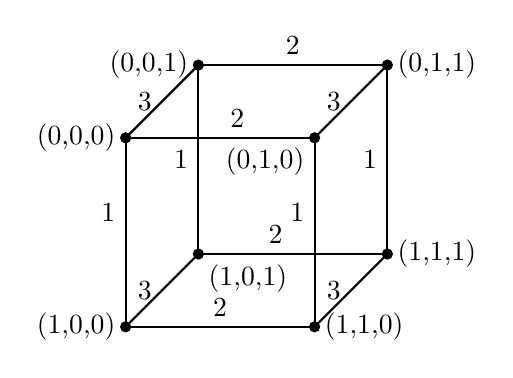
\begin{tikzpicture}[thick,scale=0.2]
\coordinate[label={180:\text{(1,0,0)}}] (UVL) at (0,0,12);
\coordinate[label={0:\text{(1,1,0)}}] (UVR) at (12,0,12);
\coordinate[label={180:\text{(0,0,0)}}] (OVL) at (0,12,12);
\coordinate[label={-120:\text{(0,1,0)}}] (OVR) at (12,12,12);
\coordinate[label={-86:\text{(1,0,1)}}] (UHL) at (0,0,0);
\coordinate[label={0:\text{(1,1,1)}}] (UHR) at (12,0,0);
\coordinate[label={180:\text{(0,0,1)}}] (OHL) at (0,12,0);
\coordinate[label={0:\text{(0,1,1)}}] (OHR) at (12,12,0);

\draw[fill=black] (UVL) circle (8pt);
\draw[fill=black] (UVR) circle (8pt);
\draw[fill=black] (OVL) circle (8pt);
\draw[fill=black] (OVR) circle (8pt);
\draw[fill=black] (UHL) circle (8pt);
\draw[fill=black] (UHR) circle (8pt);
\draw[fill=black] (OHL) circle (8pt);
\filldraw[color=black] (OHR) circle (8pt);

\draw (UVL) -- node[above] {2} (UVR);
\draw (UVL) -- node[above left] {1} (OVL);
\draw (UVL) -- node[left] {3} (UHL);
\draw (OVR) -- node[above right] {2} (OVL);
\draw (OVR) -- node[left] {3} (OHR);
\draw (OVR) -- node[above left] {1} (UVR);
\draw (OHL) -- node[left] {3} (OVL);
\draw (OHL) -- node[above] {2} (OHR);
\draw (OHL) -- node[left] {1} (UHL);
\draw (UHR) -- node[left] {3} (UVR);
\draw (UHR) -- node[left] {1} (OHR);
\draw (UHR) -- node[above left] {2} (UHL);
\end{tikzpicture}
\caption{Ausgangssituation des \textit{cheating husbands}-Rätsels}
\label{ausgang}
\end{figure}

In der graphischen Darstellung kann man gut die Symmetrie des Problems erkennen.
Die i-te Ehefrau kann die Zustände nicht unterscheiden, dessen Werte nur an der i-ten Stelle variieren.
So kann beispielsweise die erste Ehefrau die Situationen (0,0,0) und (1,0,0) nicht voneinander unterscheiden, da sie nicht weiß, ob ihr eigener Ehemann untreu war. Gleiches gilt für die Zustände (0,0,1) zu (1,0,1), (0,1,0) zu (1,1,0) und (0,1,1) zu (1,1,1).

Gehen wir nun davon aus, dass der zweite und dritte Ehemann untreu waren und wir uns somit im Zustand (0,1,1) befinden.
Nachdem die Königin ihre Ansprache gehalten hat, verändert sich die Kripke-Struktur, wie in Abbildung \ref{nachAnsprache} gezeigt.

\begin{figure}
	\centering
	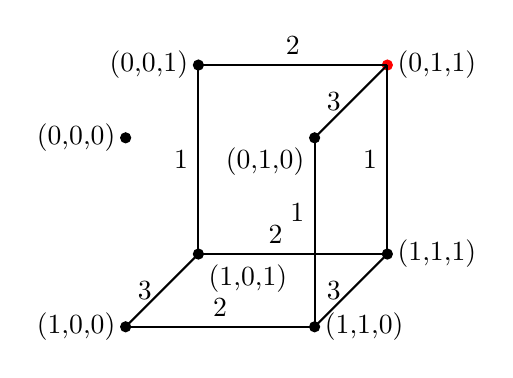
\begin{tikzpicture}[thick,scale=0.2]
	\coordinate[label={180:\text{(1,0,0)}}] (UVL) at (0,0,12);
	\coordinate[label={0:\text{(1,1,0)}}] (UVR) at (12,0,12);
	\coordinate[label={180:\text{(0,0,0)}}] (OVL) at (0,12,12);
	\coordinate[label={-120:\text{(0,1,0)}}] (OVR) at (12,12,12);
	\coordinate[label={-86:\text{(1,0,1)}}] (UHL) at (0,0,0);
	\coordinate[label={0:\text{(1,1,1)}}] (UHR) at (12,0,0);
	\coordinate[label={180:\text{(0,0,1)}}] (OHL) at (0,12,0);
	\coordinate[label={0:\text{(0,1,1)}}] (OHR) at (12,12,0);
	
	\draw[fill=black] (UVL) circle (8pt);
	\draw[fill=black] (UVR) circle (8pt);
	\draw[fill=black] (OVL) circle (8pt);
	\draw[fill=black] (OVR) circle (8pt);
	\draw[fill=black] (UHL) circle (8pt);
	\draw[fill=black] (UHR) circle (8pt);
	\draw[fill=black] (OHL) circle (8pt);
	\filldraw[color=red] (OHR) circle (8pt);
	
	\draw (UVL) -- node[above] {2} (UVR);

	\draw (UVL) -- node[left] {3} (UHL);

	\draw (OVR) -- node[left] {3} (OHR);
	\draw (OVR) -- node[above left] {1} (UVR);
	
	\draw (OHL) -- node[above] {2} (OHR);
	\draw (OHL) -- node[left] {1} (UHL);
	\draw (UHR) -- node[left] {3} (UVR);
	\draw (UHR) -- node[left] {1} (OHR);
	\draw (UHR) -- node[above left] {2} (UHL);
	\end{tikzpicture}
	\caption{Ausgangssituation des \textit{cheating husbands}-Rätsels}
	\label{nachAnsprache}
\end{figure}

Da es nach der Ansprache das gemeinsame Wissen gibt, dass es mindestens einen untreuen Ehemann in Atlantis gibt, kann der Zustand (0,0,0) von allen Ehefrauen ausgeschlossen werden.

$E^{k}(\phi)$ anhand eines Radiuses verdeutlichen